% Options for packages loaded elsewhere
\PassOptionsToPackage{unicode}{hyperref}
\PassOptionsToPackage{hyphens}{url}
\documentclass[
  ignorenonframetext,
  aspectratio=169,
]{beamer}
\newif\ifbibliography
\usepackage{pgfpages}
\setbeamertemplate{caption}[numbered]
\setbeamertemplate{caption label separator}{: }
\setbeamercolor{caption name}{fg=normal text.fg}
\beamertemplatenavigationsymbolsempty
% remove section numbering
\setbeamertemplate{part page}{
  \centering
  \begin{beamercolorbox}[sep=16pt,center]{part title}
    \usebeamerfont{part title}\insertpart\par
  \end{beamercolorbox}
}
\setbeamertemplate{section page}{
  \centering
  \begin{beamercolorbox}[sep=12pt,center]{section title}
    \usebeamerfont{section title}\insertsection\par
  \end{beamercolorbox}
}
\setbeamertemplate{subsection page}{
  \centering
  \begin{beamercolorbox}[sep=8pt,center]{subsection title}
    \usebeamerfont{subsection title}\insertsubsection\par
  \end{beamercolorbox}
}
% Prevent slide breaks in the middle of a paragraph
\widowpenalties 1 10000
\raggedbottom
\AtBeginPart{
  \frame{\partpage}
}
\AtBeginSection{
  \ifbibliography
  \else
    \frame{\sectionpage}
  \fi
}
\AtBeginSubsection{
  \frame{\subsectionpage}
}
\usepackage{iftex}
\ifPDFTeX
  \usepackage[T1]{fontenc}
  \usepackage[utf8]{inputenc}
  \usepackage{textcomp} % provide euro and other symbols
\else % if luatex or xetex
  \usepackage{unicode-math} % this also loads fontspec
  \defaultfontfeatures{Scale=MatchLowercase}
  \defaultfontfeatures[\rmfamily]{Ligatures=TeX,Scale=1}
\fi
\usepackage{lmodern}
\ifPDFTeX\else
  % xetex/luatex font selection
\fi
% Use upquote if available, for straight quotes in verbatim environments
\IfFileExists{upquote.sty}{\usepackage{upquote}}{}
\IfFileExists{microtype.sty}{% use microtype if available
  \usepackage[]{microtype}
  \UseMicrotypeSet[protrusion]{basicmath} % disable protrusion for tt fonts
}{}
\makeatletter
\@ifundefined{KOMAClassName}{% if non-KOMA class
  \IfFileExists{parskip.sty}{%
    \usepackage{parskip}
  }{% else
    \setlength{\parindent}{0pt}
    \setlength{\parskip}{6pt plus 2pt minus 1pt}}
}{% if KOMA class
  \KOMAoptions{parskip=half}}
\makeatother
\usepackage{longtable,booktabs,array}
\usepackage{caption}
\captionsetup[table]{skip=6pt}
\newcounter{none} % for unnumbered tables
\usepackage{calc} % for calculating minipage widths
\usepackage{caption}
% Make caption package work with longtable
\makeatletter
\def\fnum@table{\tablename~\thetable}
\makeatother
\usepackage{graphicx}
\makeatletter
\newsavebox\pandoc@box
\newcommand*\pandocbounded[1]{% scales image to fit in text height/width
  \sbox\pandoc@box{#1}%
  \Gscale@div\@tempa{\textheight}{\dimexpr\ht\pandoc@box+\dp\pandoc@box\relax}%
  \Gscale@div\@tempb{\linewidth}{\wd\pandoc@box}%
  \ifdim\@tempb\p@<\@tempa\p@\let\@tempa\@tempb\fi% select the smaller of both
  \ifdim\@tempa\p@<\p@\scalebox{\@tempa}{\usebox\pandoc@box}%
  \else\usebox{\pandoc@box}%
  \fi%
}
% Set default figure placement to htbp
\def\fps@figure{htbp}
\makeatother
\setlength{\emergencystretch}{3em} % prevent overfull lines
\providecommand{\tightlist}{%
  \setlength{\itemsep}{0pt}\setlength{\parskip}{0pt}}
% Auto-generated by infrastructure/rendering/_pdf_latex_helpers.py::extract_math_font_preamble.
% Minimal header passed to Pandoc via -H so Beamer slides pick up the same math font
% as the combined-PDF path. Adjust the manuscript's preamble.md to change the font globally.
\usepackage{unicode-math}
\setmathfont{latinmodern-math.otf}

% Manuscript macro/package fallbacks (newcommand -> providecommand).
% Core mathematics
\usepackage{amsmath}
\usepackage{amssymb}
% Document layout
% Tables
\usepackage{booktabs}
% Caption styling (booktabs already loaded above). Small caption font with a
% bold label ("Figure 1", "Table 2") gives the math/figure-heavy layout a
% consistent, journal-like caption rhythm without fighting pandoc-crossref —
% pandoc emits standard \caption{}, and caption/captionsetup only restyle it.
% ── Theorem environments ─────────────────────────────────────────────────
% amsthm is loaded above. The FedGVI<->Friston bridge is stated as a small
% number of theorems/definitions/lemmas/propositions/corollaries; sharing one
% counter (definition/lemma/proposition/corollary all step the `theorem`
% counter) gives a single monotone numbering 1, 2, 3, ... across all kinds, so
% authors can reference them as Theorem 1, Definition 2, Corollary 3 without a
% per-kind counter drifting out of order. Plain style for theorem-like results,
% definition style (upright body) for definitions.
% (algorithm2e intentionally not loaded: this manuscript states results as
% numbered amsthm Theorems/Definitions, not algorithm2e pseudocode.)
% Code listings
\usepackage{listings}
% Typography and formatting
% (siunitx intentionally not loaded: no \SI/\num units appear in this manuscript.)
% Cross-references and citations
% (cleveref and titlesec intentionally not loaded: unavailable in this TeX tree
% and not required. Cross-references resolve through pandoc-crossref's own
% \ref-style names — no \cref appears — and section heading styling falls back
% to the pandoc/LaTeX defaults.)
% ── TeX Live Basic-compatible mono font for code listings ────────────
% Latin Modern Mono is bundled with TeX Live Basic and keeps the manuscript
% renderable on minimal TeX installations. Mathematical Unicode coverage is
% provided separately by Latin Modern Math below, so the code font does not
% need a private JuliaMono installation.
%
% Use the TeX font filename rather than the system-family name: the minimal
% TeX Live fontconfig database may not register the OpenType family even though
% kpsewhich can resolve the bundled files.
% Math font for unicode-math: Latin Modern Math (TeX Live) has full BMP
% coverage including U+2223 (\mid), U+226A/226B (\ll/\gg), and the Greek/
% blackboard letters used in equations. Without an explicit \setmathfont,
% unicode-math falls back to lmroman text font which lacks several glyphs
% and emits "Missing character" warnings on every \mid in math mode.

% Slide layout defaults for warning-clean scientific decks.
\usepackage{etoolbox}
\IfFileExists{xurl.sty}{\usepackage{xurl}}{}
\IfFileExists{seqsplit.sty}{\usepackage{seqsplit}}{\newcommand{\seqsplit}[1]{#1}}
\protected\def\breakseq#1{\seqsplit{#1}}
\protected\def\breaktt#1{\begingroup\ttfamily\seqsplit{#1}\endgroup}
\setlength{\emergencystretch}{6em}
\tolerance=5000
\hbadness=10000
\hfuzz=1pt
\setlength{\tabcolsep}{2pt}
\AtBeginEnvironment{longtable}{\tiny\renewcommand{\arraystretch}{0.86}\setlength{\tabcolsep}{1pt}}
\AtBeginEnvironment{tabular}{\tiny\renewcommand{\arraystretch}{0.86}\setlength{\tabcolsep}{1pt}}
\AtBeginEnvironment{equation}{\tiny}
\AtBeginEnvironment{equation*}{\tiny}
\AtBeginEnvironment{align}{\tiny}
\AtBeginEnvironment{align*}{\tiny}
\AtBeginEnvironment{itemize}{\footnotesize}
\AtBeginEnvironment{enumerate}{\footnotesize}
\AtBeginEnvironment{description}{\footnotesize}
\setbeamerfont{caption}{size=\tiny}
\setbeamerfont{caption name}{size=\tiny}
\setbeamerfont{normal text}{size=\small}
\setbeamerfont{frametitle}{size=\small}
\setbeamerfont{section title}{size=\footnotesize}
\setbeamerfont{subsection title}{size=\footnotesize}
\setbeamertemplate{section page}{%
  \centering
  \begin{beamercolorbox}[sep=12pt,center,wd=\paperwidth]{section title}
    \parbox{0.86\paperwidth}{\centering\usebeamerfont{section title}\insertsection\par}
  \end{beamercolorbox}
}
\setbeamertemplate{subsection page}{%
  \centering
  \begin{beamercolorbox}[sep=8pt,center,wd=\paperwidth]{subsection title}
    \parbox{0.86\paperwidth}{\centering\usebeamerfont{subsection title}\insertsubsection\par}
  \end{beamercolorbox}
}
\setlength{\abovecaptionskip}{2pt}
\setlength{\belowcaptionskip}{0pt}

% Natbib and cross-reference fallbacks — slides don't load natbib
% or cleveref, but combined-PDF manuscript prose may emit these
% commands. The fallback renders citations as a bracketed key list
% and cross-references as detokenized labels so slides don't fail on
% undefined control sequences or raw underscores. \providecommand is
% a no-op if packages load later.
\providecommand{\citep}[1]{[#1]}
\providecommand{\citet}[1]{#1}
\providecommand{\citealp}[1]{#1}
\providecommand{\citeauthor}[1]{#1}
\providecommand{\citeyear}[1]{#1}
\providecommand{\cref}[1]{\texttt{\detokenize{#1}}}
\providecommand{\Cref}[1]{\texttt{\detokenize{#1}}}
\providecommand{\crefrange}[2]{\texttt{\detokenize{#1}}--\texttt{\detokenize{#2}}}
\providecommand{\Crefrange}[2]{\texttt{\detokenize{#1}}--\texttt{\detokenize{#2}}}
\providecommand{\paragraph}[1]{\textbf{#1}\ }

% Opt-in accessible presentation profile.
\setbeamerfont{normal text}{size*={20pt}{24pt}}
\setbeamerfont{frametitle}{size*={28pt}{32pt}}
\setbeamerfont{section title}{size*={28pt}{32pt}}
\setbeamerfont{subsection title}{size*={28pt}{32pt}}
\setbeamerfont{caption}{size*={16pt}{19pt}}
\setbeamerfont{caption name}{size*={16pt}{19pt}}
\setbeamerfont{itemize/enumerate body}{size*={20pt}{24pt}}
\setbeamerfont{itemize/enumerate subbody}{size*={20pt}{24pt}}
\setbeamerfont{itemize/enumerate subsubbody}{size*={20pt}{24pt}}
\setbeamerfont{itemize item}{size*={20pt}{24pt}}
\setbeamerfont{itemize subitem}{size*={20pt}{24pt}}
\setbeamerfont{itemize subsubitem}{size*={20pt}{24pt}}
\setbeamerfont{description body}{size*={20pt}{24pt}}
\setbeamerfont{description item}{size*={20pt}{24pt}}
\setbeamerfont{quote}{size*={20pt}{24pt}}
\setbeamerfont{quotation}{size*={20pt}{24pt}}
\AtBeginEnvironment{longtable}{\fontsize{20pt}{24pt}\selectfont}
\AtBeginEnvironment{tabular}{\fontsize{20pt}{24pt}\selectfont}
\AtBeginEnvironment{equation}{\fontsize{20pt}{24pt}\selectfont}
\AtBeginEnvironment{equation*}{\fontsize{20pt}{24pt}\selectfont}
\AtBeginEnvironment{align}{\fontsize{20pt}{24pt}\selectfont}
\AtBeginEnvironment{align*}{\fontsize{20pt}{24pt}\selectfont}
\AtBeginEnvironment{itemize}{\fontsize{20pt}{24pt}\selectfont}
\AtBeginEnvironment{enumerate}{\fontsize{20pt}{24pt}\selectfont}
\AtBeginEnvironment{description}{\fontsize{20pt}{24pt}\selectfont}
\AtBeginDocument{\usebeamerfont{normal text}}
\newlength{\AFSlideTableWidth}
% The fixed footer reservation is calibrated with the semantic seven-line regular-body budget.
\setbeamertemplate{footline}{%
  \leavevmode\vbox{%
    \hbox{%
      \begin{beamercolorbox}[wd=\paperwidth,ht=16pt,dp=3pt,center]{author in head/foot}%
        \fontsize{16pt}{19pt}\selectfont Untagged PDF derivative \textbar\ \href{../web/index.html}{HTML reader}%
      \end{beamercolorbox}%
    }%
    \vskip6pt%
  }%
}
% Accessible footer reserved height: 25pt.

\newtheorem{proposition}{Proposition}
\newtheorem{hypothesis}{Hypothesis}
\newtheorem{remark}[theorem]{Remark}
\newtheorem{axiom}{Axiom}
\newtheorem{property}{Property}
\usepackage{bookmark}
\IfFileExists{xurl.sty}{\usepackage{xurl}}{} % add URL line breaks if available
\urlstyle{same}
% fallback for those not using the hyperref driver hyperxmp:
\makeatletter
\@ifundefined{xmpquote}{\newcommand{\xmpquote}[1]{#1}}{}
\makeatother
\hypersetup{
  hidelinks,
  pdfcreator={LaTeX via pandoc}}

\author{\texorpdfstring{}{}}
\date{}

\begin{document}

\begin{frame}{Aggregation and message passing: standard pool, heuristic,
and variational server}
\protect\phantomsection\label{sec:method-aggregation}
\end{frame}

\begin{frame}[fragile]{Aggregation and message\ldots{} (part 2)}
The server step lives in \texttt{aggregation.py}, where a categorical
specialization of the active-inference belief-sharing relation (Friston
et al. 2024) and the FedGVI objective (Mildner et al. 2025) meet. Each
agent \(n\) broadcasts a categorical local posterior \(q_n(s)\) over the
shared latent factor,
\end{frame}

\begin{frame}[fragile]{Aggregation and message\ldots{} (part 3)}
optionally with a scalar base weight \(w_n\).

Two fusion rules act directly on these broadcasts, and a third --- the
objective-backed \texttt{variational\_aggregate} of
sec.~5.8.2 --- refines the second into descent on
a stated objective.
\end{frame}

\begin{frame}{Aggregation and message\ldots{} (part 4)}
The first is the \textbf{log-linear pool}, a project-local
product-of-experts consensus. In the terminology of opinion pooling it
is the logarithmic pool,
\end{frame}

\begin{frame}{Aggregation and message\ldots{} (part 5)}
a weighted geometric aggregation rule whose Bayesian-coherence
assumptions have been studied independently of active inference (Genest
and Zidek 1986; Genest et al. 1986; Carvalho et al. 2023); in
machine-learning terms it is the product-of-experts normalization of
local posteriors (Hinton 2002):
\end{frame}

\begin{frame}{Aggregation and message\ldots{} (part 6)}
\begin{equation}\tag{9}\protect\phantomsection\label{eq:log-linear-pool}{
\begin{aligned}
&\operatorname{log\_linear\_pool}(\{q_n\})\\
&\qquad = \mathrm{softmax}\!\Big(\textstyle\sum_n w_n \log q_n\Big).
\end{aligned}
}\end{equation}
\end{frame}

\begin{frame}{Aggregation and message\ldots{} (part 7)}
In the floating-point implementation, \(q_n\) denotes the admitted
posterior after input validation, lower flooring of masses, and row
normalization. The floor acts before normalization and applies to small
positive masses as well as exact zeros. The pooling formula uses those
admitted posteriors;
\end{frame}

\begin{frame}{Aggregation and message\ldots{} (part 8)}
rescaling sufficiently small raw masses can change them.

For the source bridge, fix one finite shared support \(\mathcal S\) with
\(q_n(s)>0\) for every agent and state.
\end{frame}

\begin{frame}{Aggregation and message\ldots{} (part 9)}
Suppose the inputs to Eq. 7's softmax message-combination term can be
represented as posterior log potentials \(m_n(s)=\log q_n(s)+\kappa_n\),
where \(\kappa_n\) is constant in \(s\), and use declared fixed weights
\(w_n\) that do not depend on the emerging consensus (the unweighted
case sets each \(w_n=1\)).
\end{frame}

\begin{frame}{Aggregation and message\ldots{} (part 10)}
Additive constants then cancel under softmax, giving exactly
eq.~9.
\end{frame}

\begin{frame}{Aggregation and message\ldots{} (part 11)}
This is a categorical posterior-log-potential specialization of the
source equation's message-combination term, not a reconstruction of
source message construction, self-exclusion/cavity policy, scheduling,
generative factors, or the complete protocol.
\end{frame}

\begin{frame}[fragile]{Aggregation and message\ldots{} (part 12)}
The code alias \texttt{friston\_belief\_share} names this qualified
specialization only.
\end{frame}

\begin{frame}[fragile]{Aggregation and message\ldots{} (part 13)}
The second rule is \textbf{\texttt{robust\_aggregate}}, an
iteratively-reweighted pool that discounts each agent by
\(\exp(-c\,\mathrm{KL}(q_n \,\|\, q))\) against the emerging consensus
\(q\). A confidently-wrong (contaminated) agent sits far from the
consensus,
\end{frame}

\begin{frame}{Aggregation and message\ldots{} (part 14)}
can earn a small effective weight and be suppressed in the declared
diagnostic regimes.
\end{frame}

\begin{frame}{Aggregation and message\ldots{} (part 15)}
This independently motivated rule does not transfer FedGVI's client
theorem to the server side: it is the \textbf{heuristic robustness axis}
of sec.~3.3, distinct from the per-agent rigorous
axis of sec.~5.7.
\end{frame}

\begin{frame}{Aggregation and message\ldots{} (part 16)}
It is also only an analogy to robust federated aggregation methods such
as divergence-weighted gamma-mean aggregation, geometric-median robust
aggregation, or Byzantine-tolerant gradient aggregation (Li et al. 2022;
Pillutla et al. 2022; Blanchard et al. 2017).
\end{frame}

\begin{frame}{Aggregation and message\ldots{} (part 17)}
Those methods motivate the risk surface, but they do not supply this
rule's guarantee.

The defining identity is bit-level: at zero robustness the reweighted
pool is the log-linear pool unchanged.
\end{frame}

\begin{frame}{Aggregation and message\ldots{} (part 18)}
\begin{equation}\tag{10}\protect\phantomsection\label{eq:robust-identity}{
\operatorname{robust\_aggregate}(0)
\;\equiv\;
\operatorname{log\_linear\_pool}.
}\end{equation}
\end{frame}

\begin{frame}{Aggregation and message\ldots{} (part 19)}
This is an exact project-local code identity. Under the stated
posterior-log-potential assumptions, its right-hand side specializes the
message-combination term of Eq. 7; the identity itself neither recovers
nor certifies the complete source protocol (Friston et al. 2024).
\end{frame}

\begin{frame}{Protocol map: local updates, broadcast, and server fusion}
\protect\phantomsection\label{sec:method-message-passing}
The visual map in fig.~3 makes the protocol
boundary explicit: each client updates and broadcasts a categorical
posterior; the server chooses the standard pool, heuristic, or
variational route.
\end{frame}

\begin{frame}{Protocol map (part 2)}
This is a mechanistic schematic, not an additional benchmark:
client-side FedGVI is source- conditional, server-heuristic accuracy is
conditional on declared contamination,

and the variational route owns objective/descent/raw-weight properties.
\end{frame}

\begin{frame}{Protocol map (part 3)}
\begin{figure}
\centering
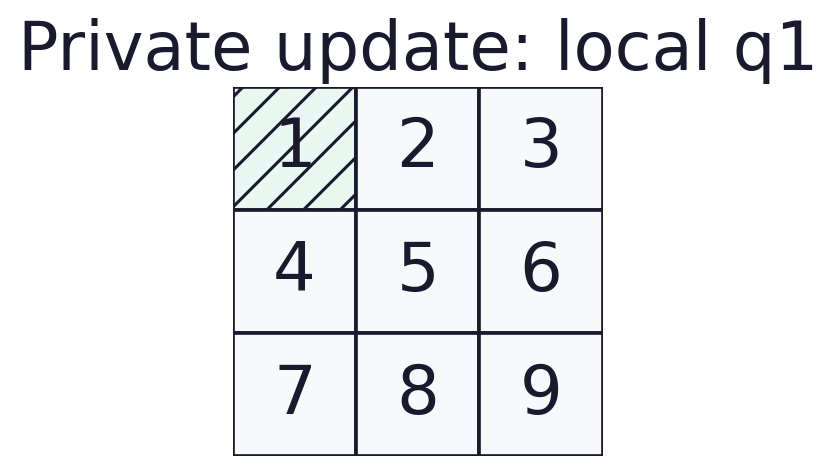
\includegraphics[keepaspectratio,width=0.98\linewidth,height=0.8\textheight,alt={Private update: local q1: nine-cell topology; cell 1 is hatched. Schematic only, no measured probability scale.}]{../figures/message_passing.slide-posterior-1.png}
\refstepcounter{figure}\label{fig:message-passing-slide-panel-1}
\end{figure}
\end{frame}

\begin{frame}{Protocol map (part 4)}
\begin{figure}
\centering
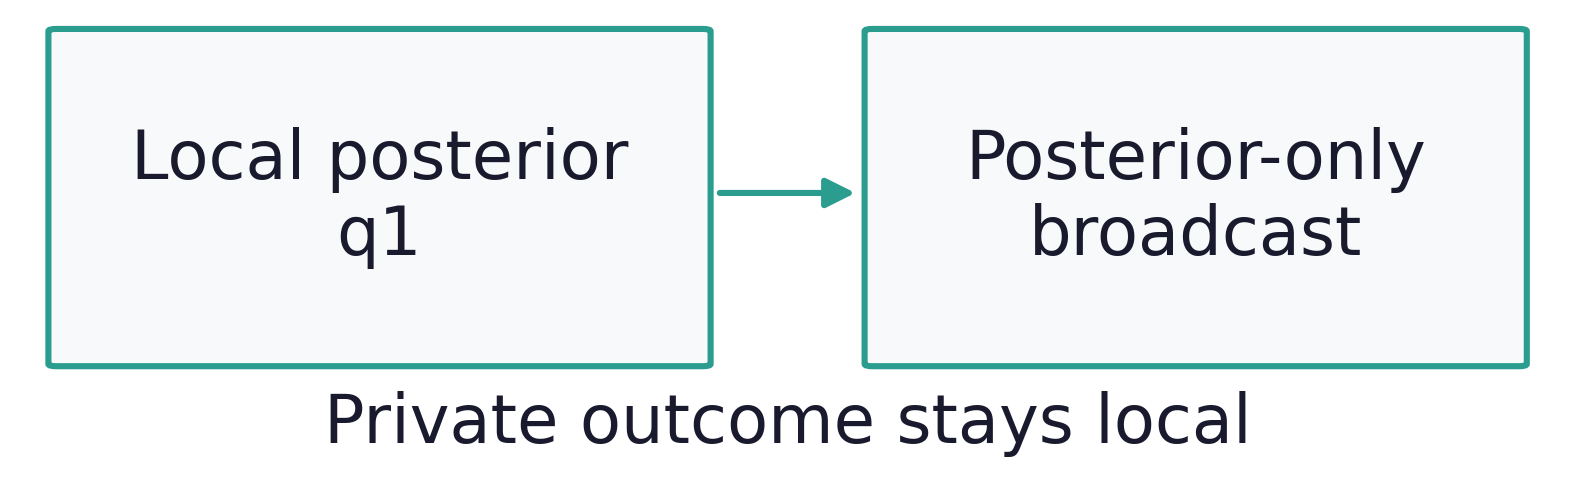
\includegraphics[keepaspectratio,width=0.98\linewidth,height=0.8\textheight,alt={Local posterior q1 → Posterior-only broadcast: Private outcome stays local; data\_dependency.}]{../figures/message_passing.slide-broadcast-1.png}
\refstepcounter{figure}\label{fig:message-passing-slide-panel-2}
\end{figure}
\end{frame}

\begin{frame}{Protocol map (part 5)}
\begin{figure}
\centering
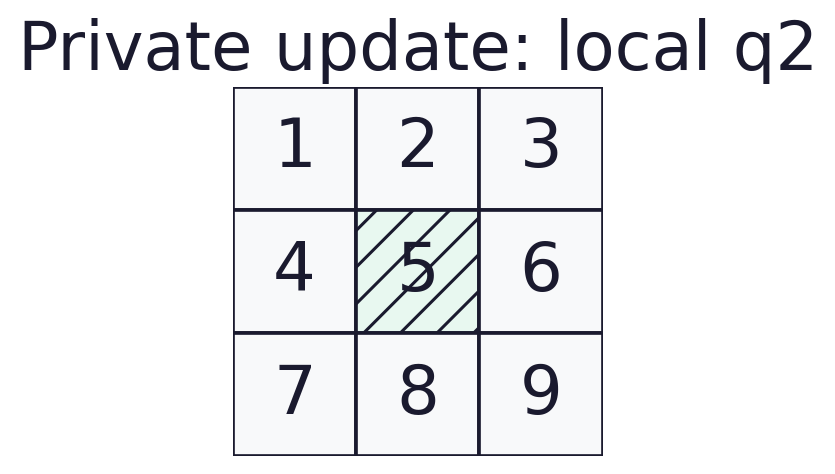
\includegraphics[keepaspectratio,width=0.98\linewidth,height=0.8\textheight,alt={Private update: local q2: nine-cell topology; cell 5 is hatched. Schematic only, no measured probability scale.}]{../figures/message_passing.slide-posterior-2.png}
\refstepcounter{figure}\label{fig:message-passing-slide-panel-3}
\end{figure}
\end{frame}

\begin{frame}{Protocol map (part 6)}
\begin{figure}
\centering
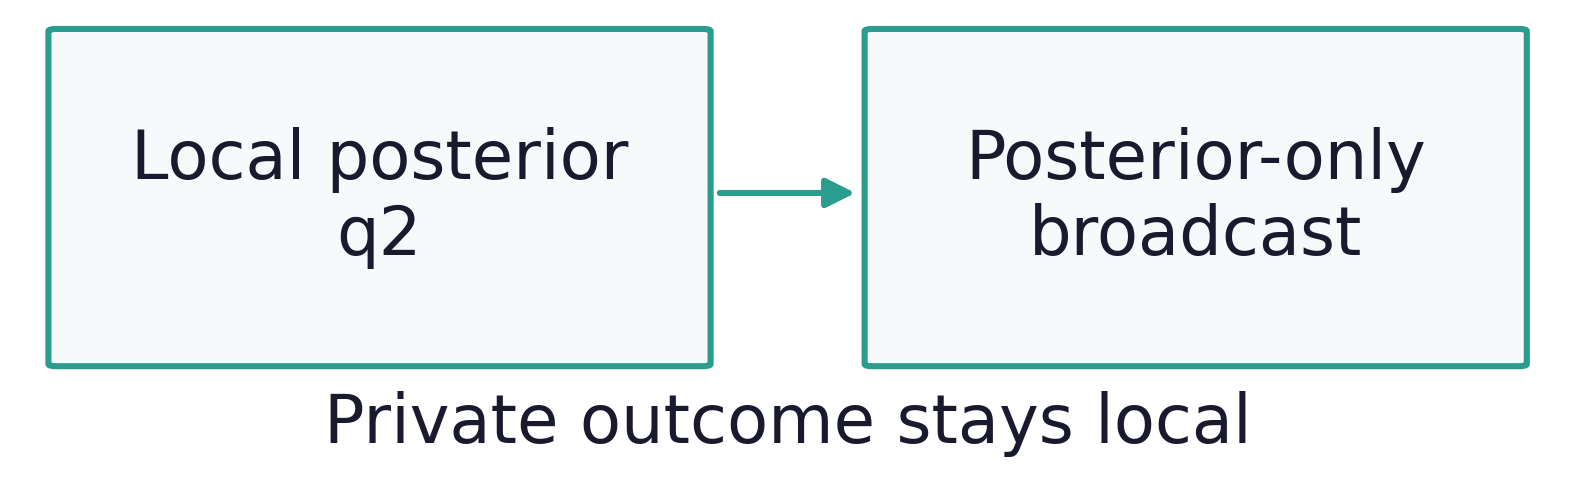
\includegraphics[keepaspectratio,width=0.98\linewidth,height=0.8\textheight,alt={Local posterior q2 → Posterior-only broadcast: Private outcome stays local; data\_dependency.}]{../figures/message_passing.slide-broadcast-2.png}
\refstepcounter{figure}\label{fig:message-passing-slide-panel-4}
\end{figure}
\end{frame}

\begin{frame}{Protocol map (part 7)}
\begin{figure}
\centering
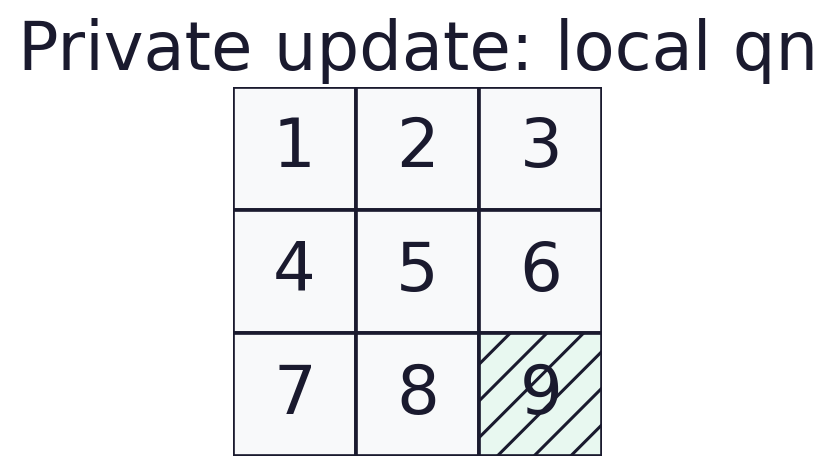
\includegraphics[keepaspectratio,width=0.98\linewidth,height=0.8\textheight,alt={Private update: local qn: nine-cell topology; cell 9 is hatched. Schematic only, no measured probability scale.}]{../figures/message_passing.slide-posterior-n.png}
\refstepcounter{figure}\label{fig:message-passing-slide-panel-5}
\end{figure}
\end{frame}

\begin{frame}{Protocol map (part 8)}
\begin{figure}
\centering
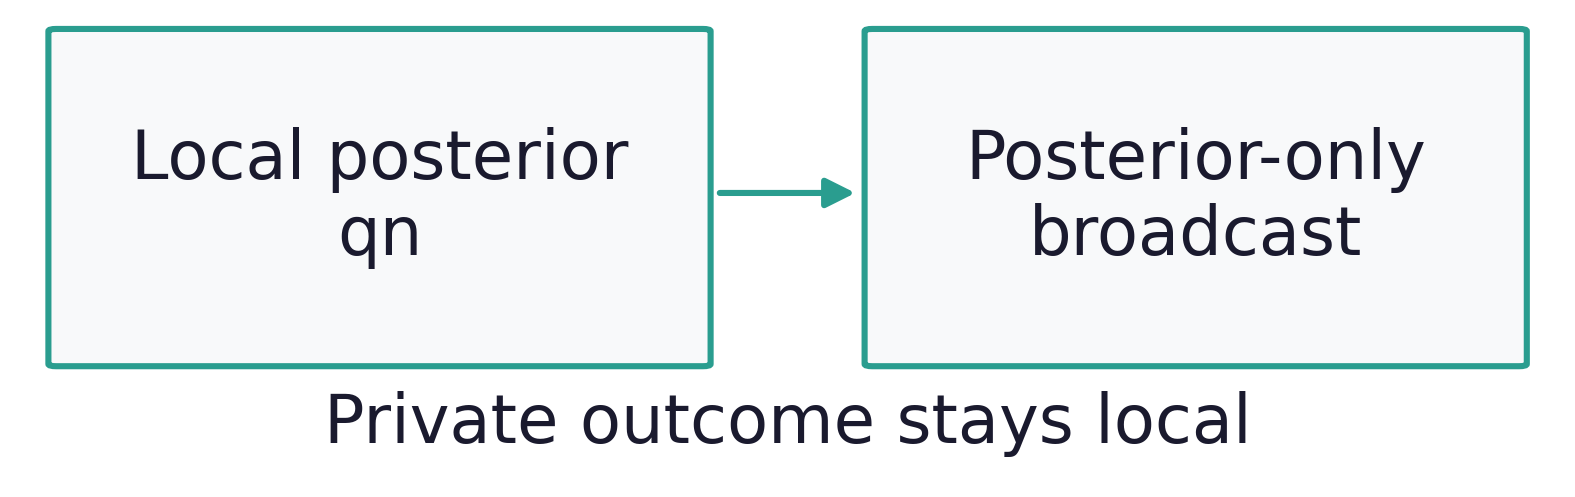
\includegraphics[keepaspectratio,width=0.98\linewidth,height=0.8\textheight,alt={Local posterior qn → Posterior-only broadcast: Private outcome stays local; data\_dependency.}]{../figures/message_passing.slide-broadcast-n.png}
\refstepcounter{figure}\label{fig:message-passing-slide-panel-6}
\end{figure}
\end{frame}

\begin{frame}{Protocol map (part 9)}
\begin{figure}
\centering

\includegraphics[keepaspectratio,width=0.98\linewidth,height=0.8\textheight,alt={Client route: NLL/KLD/β = 0 is a project recovery identity.}]{../figures/message_passing.slide-client-recovery.png}
\refstepcounter{figure}\label{fig:message-passing-slide-panel-7}
\end{figure}
\end{frame}

\begin{frame}{Protocol map (part 10)}
\begin{figure}
\centering
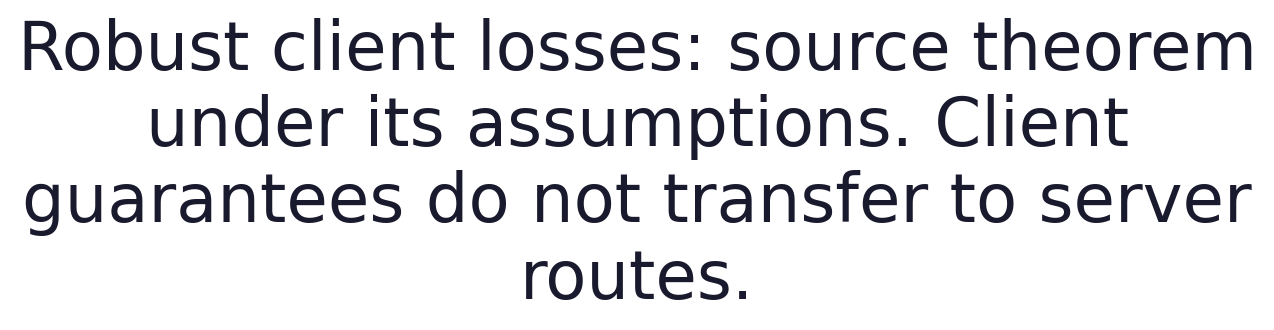
\includegraphics[keepaspectratio,width=0.98\linewidth,height=0.8\textheight,alt={Robust client losses: source theorem under its assumptions. Client guarantees do not transfer to server routes.}]{../figures/message_passing.slide-client-theorem.png}
\refstepcounter{figure}\label{fig:message-passing-slide-panel-8}
\end{figure}
\end{frame}

\begin{frame}{Protocol map (part 11)}
\begin{figure}
\centering

\includegraphics[keepaspectratio,width=0.98\linewidth,height=0.8\textheight,alt={Protocol-v1 payload: categorical posterior q(n). No private outcome o(n) is broadcast.}]{../figures/message_passing.slide-transport.png}
\refstepcounter{figure}\label{fig:message-passing-slide-panel-9}
\end{figure}
\end{frame}

\begin{frame}{Protocol map (part 12)}
\begin{figure}
\centering
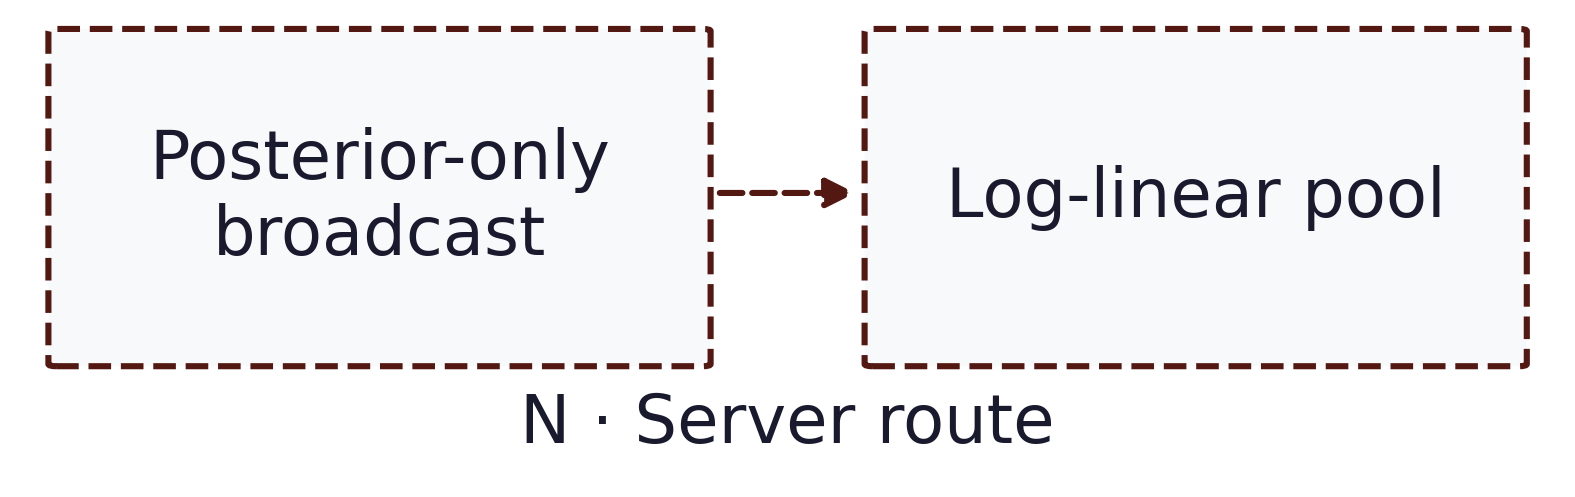
\includegraphics[keepaspectratio,width=0.98\linewidth,height=0.8\textheight,alt={Posterior-only broadcast → Log-linear pool: N · Server route; naive.}]{../figures/message_passing.slide-route-naive.png}
\refstepcounter{figure}\label{fig:message-passing-slide-panel-10}
\end{figure}
\end{frame}

\begin{frame}{Protocol map (part 13)}
\begin{figure}
\centering
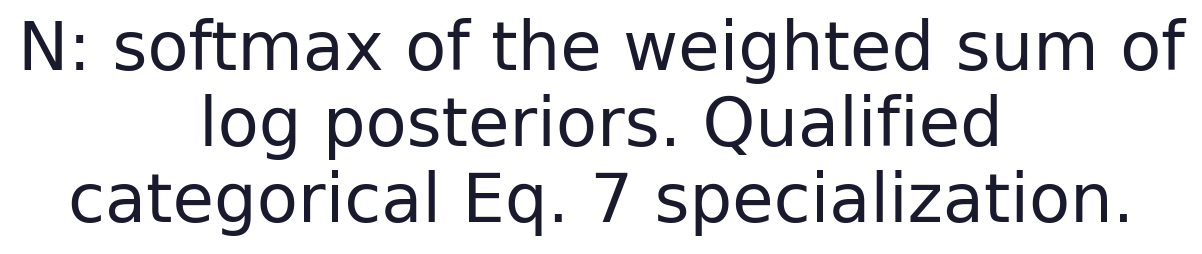
\includegraphics[keepaspectratio,width=0.98\linewidth,height=0.8\textheight,alt={N: softmax of the weighted sum of log posteriors. Qualified categorical Eq. 7 specialization.}]{../figures/message_passing.slide-owner-naive.png}
\refstepcounter{figure}\label{fig:message-passing-slide-panel-11}
\end{figure}
\end{frame}

\begin{frame}{Protocol map (part 14)}
\begin{figure}
\centering
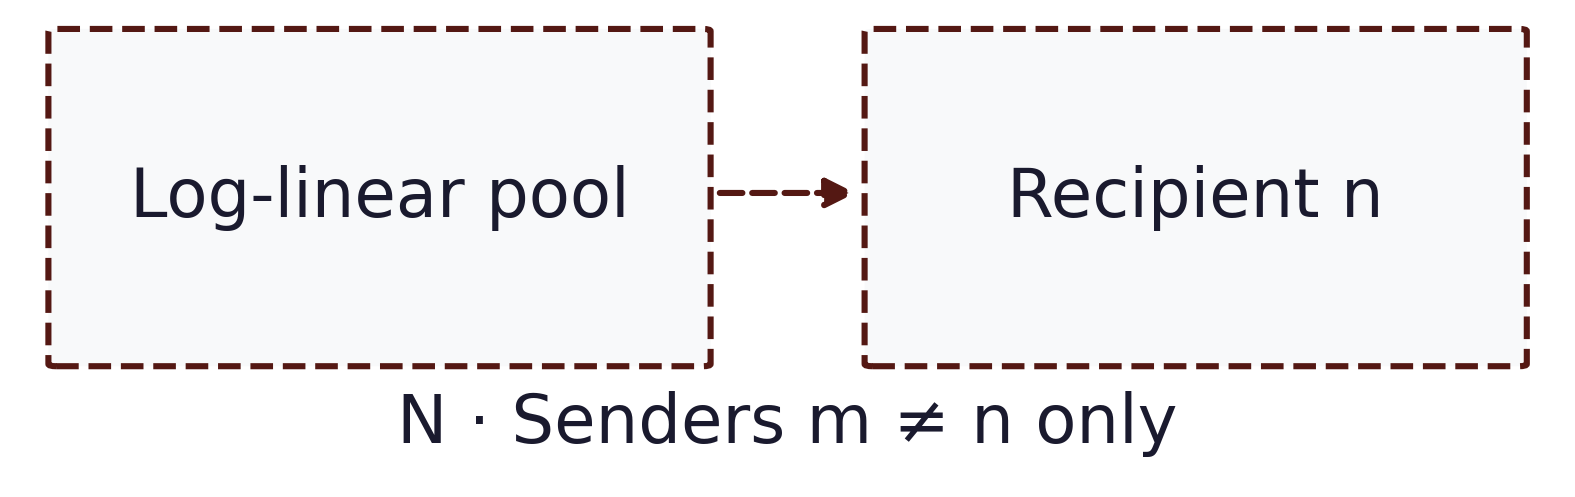
\includegraphics[keepaspectratio,width=0.98\linewidth,height=0.8\textheight,alt={Log-linear pool → Recipient n: N · Senders m ≠ n only; naive.}]{../figures/message_passing.slide-return-naive.png}
\refstepcounter{figure}\label{fig:message-passing-slide-panel-12}
\end{figure}
\end{frame}

\begin{frame}{Protocol map (part 15)}
\begin{figure}
\centering
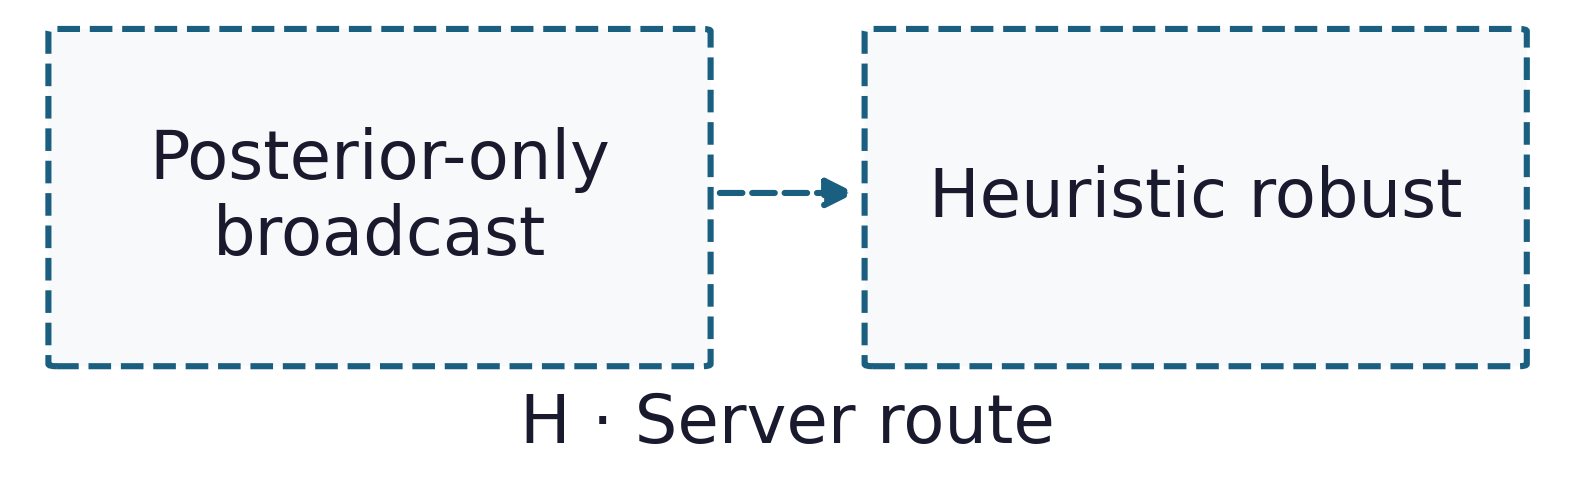
\includegraphics[keepaspectratio,width=0.98\linewidth,height=0.8\textheight,alt={Posterior-only broadcast → Heuristic robust: H · Server route; heuristic\_robust.}]{../figures/message_passing.slide-route-heuristic-robust.png}
\refstepcounter{figure}\label{fig:message-passing-slide-panel-13}
\end{figure}
\end{frame}

\begin{frame}{Protocol map (part 16)}
\begin{figure}
\centering
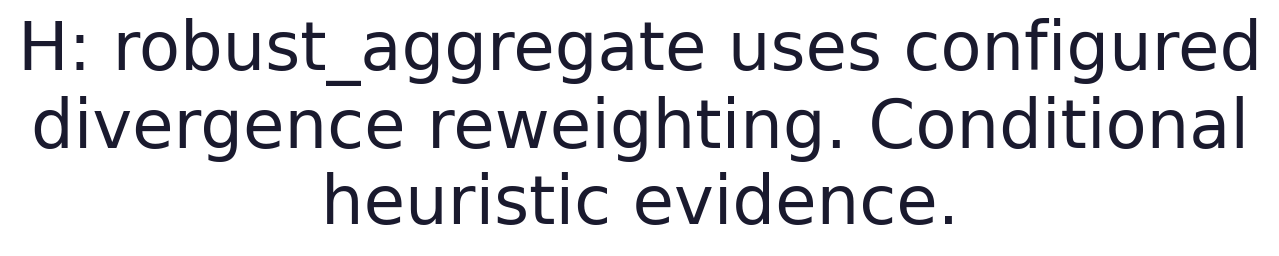
\includegraphics[keepaspectratio,width=0.98\linewidth,height=0.8\textheight,alt={H: robust\_aggregate uses configured divergence reweighting. Conditional heuristic evidence.}]{../figures/message_passing.slide-owner-heuristic-robust.png}
\refstepcounter{figure}\label{fig:message-passing-slide-panel-14}
\end{figure}
\end{frame}

\begin{frame}{Protocol map (part 17)}
\begin{figure}
\centering
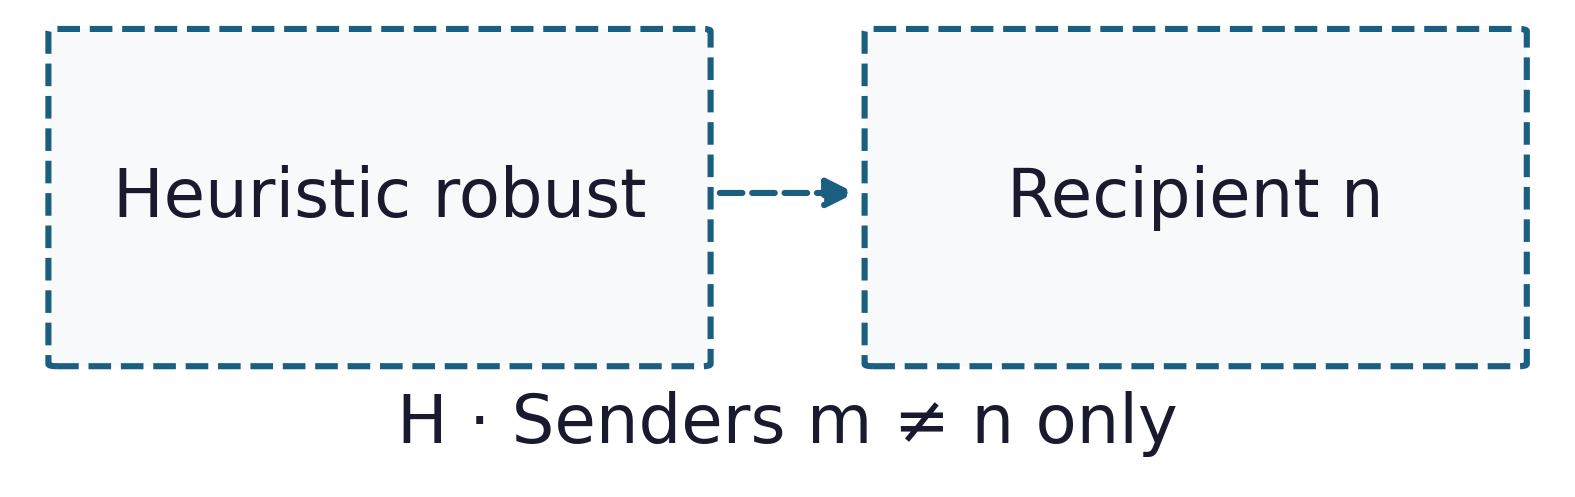
\includegraphics[keepaspectratio,width=0.98\linewidth,height=0.8\textheight,alt={Heuristic robust → Recipient n: H · Senders m ≠ n only; heuristic\_robust.}]{../figures/message_passing.slide-return-heuristic-robust.png}
\refstepcounter{figure}\label{fig:message-passing-slide-panel-15}
\end{figure}
\end{frame}

\begin{frame}{Protocol map (part 18)}
\begin{figure}
\centering
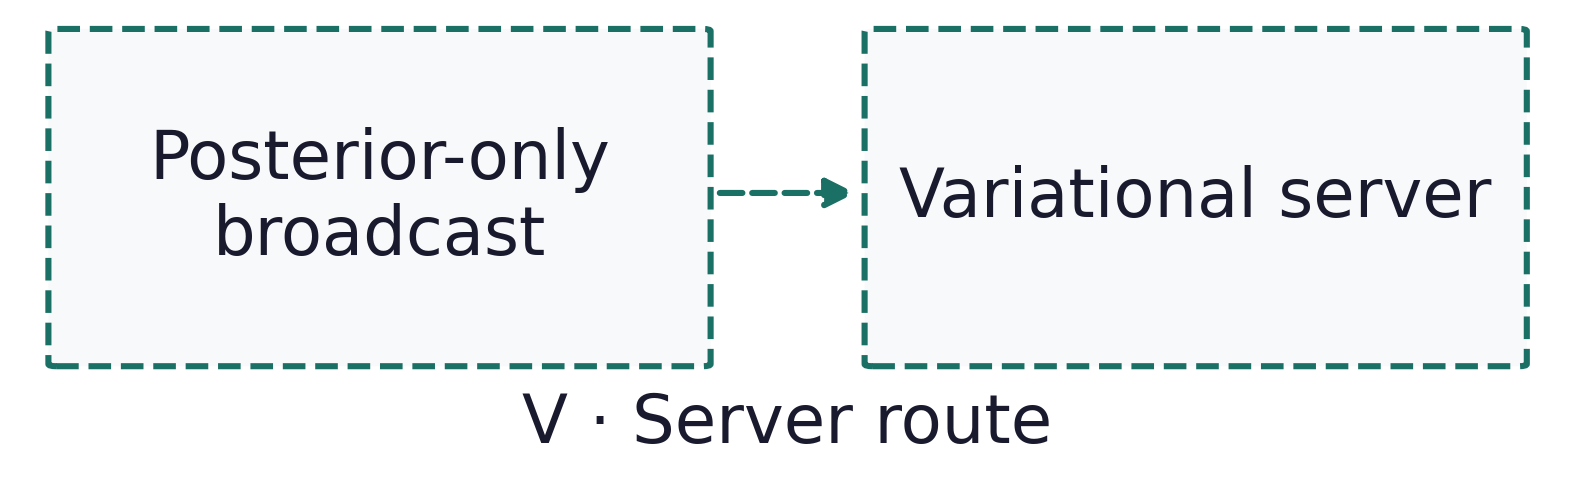
\includegraphics[keepaspectratio,width=0.98\linewidth,height=0.8\textheight,alt={Posterior-only broadcast → Variational server: V · Server route; variational.}]{../figures/message_passing.slide-route-variational.png}
\refstepcounter{figure}\label{fig:message-passing-slide-panel-16}
\end{figure}
\end{frame}

\begin{frame}{Protocol map (part 19)}
\begin{figure}
\centering
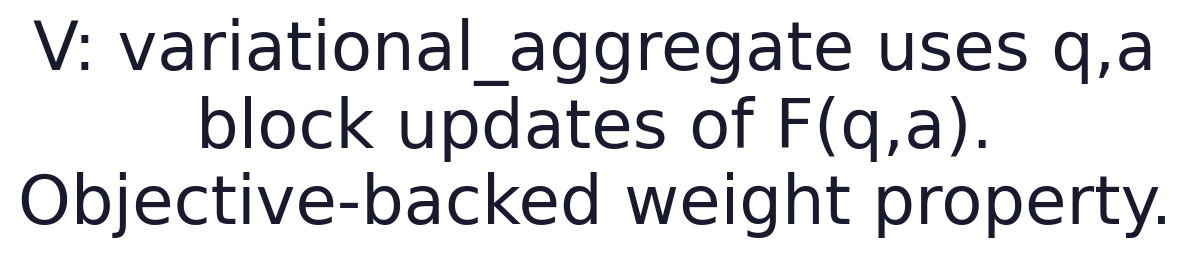
\includegraphics[keepaspectratio,width=0.98\linewidth,height=0.8\textheight,alt={V: variational\_aggregate uses q,a block updates of F(q,a). Objective-backed weight property.}]{../figures/message_passing.slide-owner-variational.png}
\refstepcounter{figure}\label{fig:message-passing-slide-panel-17}
\end{figure}
\end{frame}

\begin{frame}{Protocol map (part 20)}
\begin{figure}
\centering
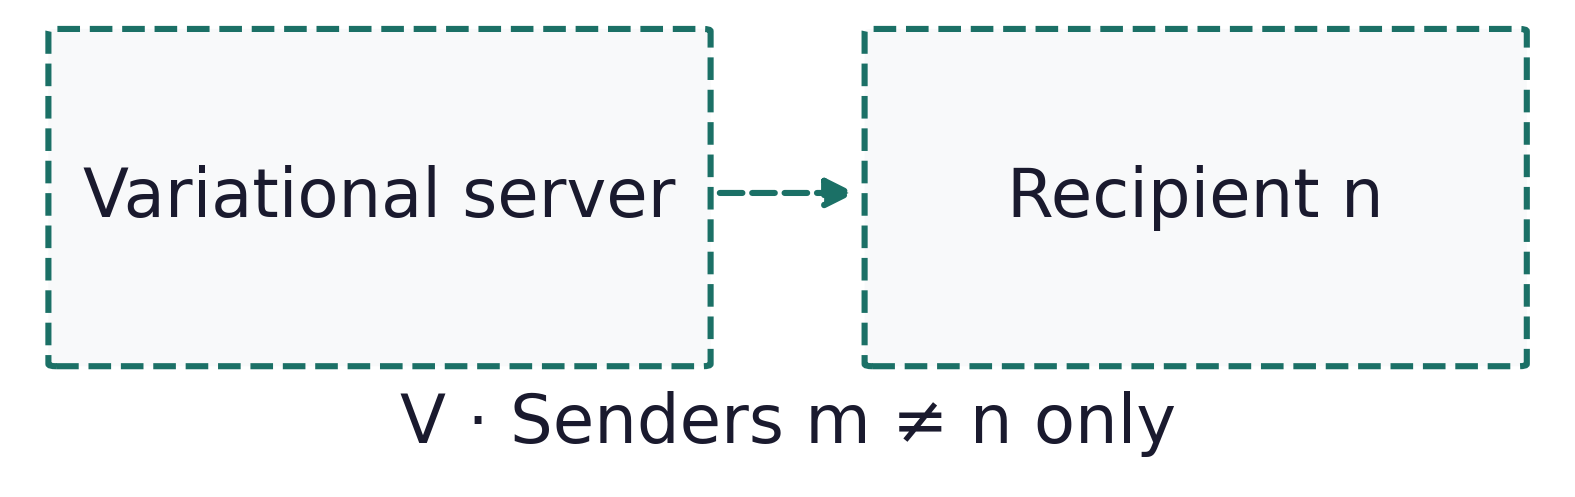
\includegraphics[keepaspectratio,width=0.98\linewidth,height=0.8\textheight,alt={Variational server → Recipient n: V · Senders m ≠ n only; variational.}]{../figures/message_passing.slide-return-variational.png}
\refstepcounter{figure}\label{fig:message-passing-slide-panel-18}
\end{figure}
\end{frame}

\begin{frame}{Protocol map (part 21)}
\begin{figure}
\centering
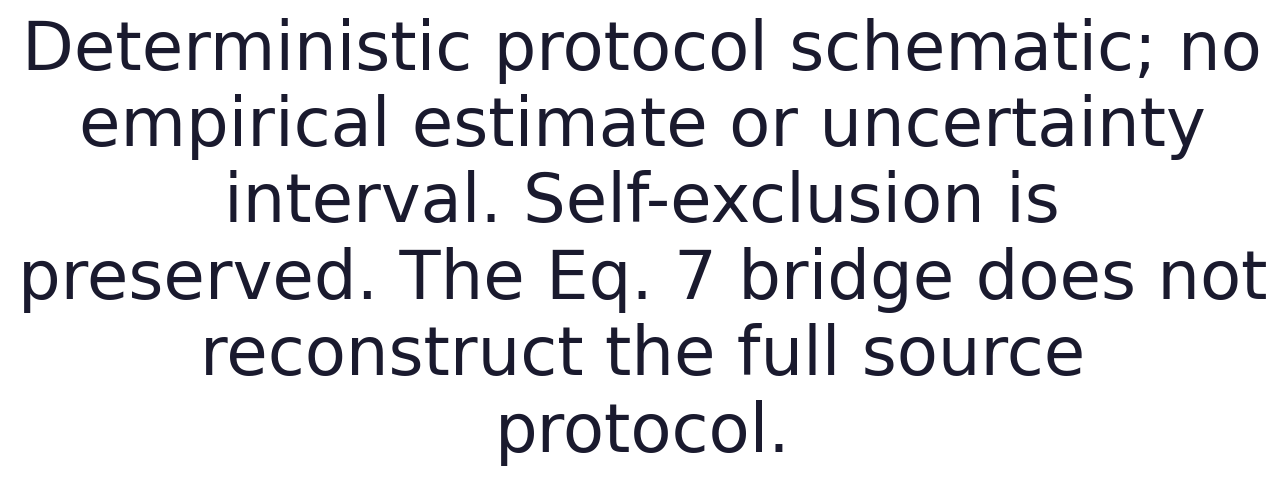
\includegraphics[keepaspectratio,width=0.98\linewidth,height=0.8\textheight,alt={Deterministic protocol schematic; no empirical estimate or uncertainty interval. Self-exclusion is preserved. The Eq. 7 bridge does not reconstruct the full source protocol.}]{../figures/message_passing.slide-scope.png}
\refstepcounter{figure}\label{fig:message-passing-slide-panel-19}
\end{figure}
\end{frame}

\begin{frame}{Protocol map (part 22)}
\begin{theorem}[Categorical combination and recovery]\label{thm:belief-sharing-recovery}
For finite $\mathcal S$ and $q_n(s)>0$, take Eq. 7 inputs
$m_n(s)=\log q_n(s)+\kappa_n$, with state-constant $\kappa_n$ and fixed $w_n$.
$\operatorname{softmax}(\sum_n w_n m_n)$ equals
(9). At $c=0$, the server returns it by
(10). This identifies categorical combination and
recovery only, not the protocol or $c>0$ behavior.
\end{theorem}
\end{frame}

\begin{frame}{Protocol map (part 23)}
At \(c=0\), every reweighting multiplier is \(\exp(0)=1\), the iteration
is skipped, and the same pool code path returns.
\end{frame}

\begin{frame}{Protocol map (part 24)}
\begin{corollary}[Closed-form Bayes recovery]\label{cor:closed-form-bayes}
With KL/NLL, the posterior of (2) is the prior-times-likelihood
product in (11). Thus
\texttt{generalized\_posterior(KLD, NLL)} reproduces Bayes. Under Theorem
5, pooling those posteriors specializes Eq. 7's
categorical combination term, not its complete protocol.
\end{corollary}
\end{frame}

\begin{frame}{Protocol map (part 25)}
\begin{equation}\tag{11}\protect\phantomsection\label{eq:standard-bayes}{
q^\ast(s) \;\propto\; \pi_0(s)\,\textstyle\prod_i p(o_i\mid s),
}\end{equation}
\end{frame}

\begin{frame}{Protocol map (part 26)}
Pooling gives the project log-linear pool of
eq.~9.
\end{frame}

\begin{frame}[fragile]{Protocol map (part 27)}
The largest observed discrepancy between
\texttt{robust\_aggregate(robustness=0)} and \texttt{log\_linear\_pool}
is 0 --- bit-identical, since the zero-robustness branch runs the same
code path --- and between \texttt{generalized\_posterior(KLD,\ NLL)} and
the analytic Bayes posterior is 5.55e-17,
\end{frame}

\begin{frame}{Protocol map (part 28)}
exact to machine precision (about one ULP); both are reported in
sec.~7.1, so eq.~10 and
eq.~11 are verified identities rather than
approximations.
\end{frame}

\begin{frame}[fragile]{Protocol map (part 29)}
The honesty contract binds at exactly this point. The recovery theorem
and its corollary cover only the recovery identity and the per-agent
rigorous axis of sec.~5.7; no statement \emph{about
\texttt{robust\_aggregate}} transfers a bounded-influence guarantee to
that divergence-reweighting,
\end{frame}

\begin{frame}{Protocol map (part 30)}
whose positive property is the \(\texttt{robustness}=0\) limit of
eq.~10.
\end{frame}

\begin{frame}{Protocol map (part 31)}
A scoped no-go rejects a declared separable objective class without
supplying a broader objective certificate. The per-agent influence
weights that the heuristic produces under contamination are
\emph{illustrated}, not guaranteed, in fig.~15.
\end{frame}

\begin{frame}{Protocol map (part 32)}
The separate fig.~18 is an exploratory
generalized-Bayes point-estimate logistic-regression baseline comparing
joint NLL/L2 and RCCE/L2 configurations. Because both loss and shrinkage
differ, it does not isolate an RCCE-only effect or test the genuine
per-client FedGVI property,
\end{frame}

\begin{frame}{Protocol map (part 33)}
which remains source-conditional in sec.~5.7.

The next subsection closes this exact gap on the server side with a
\emph{different}, objective-backed aggregator.
\end{frame}

\begin{frame}{Variational aggregation with objective-backed weight
control}
\protect\phantomsection\label{sec:method-variational}
The related server construction becomes a genuinely variational rule by
replacing the heuristic's reverse-KL weight update with a forward
cross-entropy update. For \(c>0\) and \(\lambda>0\),
\end{frame}

\begin{frame}{Variational aggregation with\ldots{} (part 2)}
treat the consensus \(q\) and a vector of effective weights
\(a = (a_n)\) as joint variational parameters and define the
\textbf{aggregation free energy}
\end{frame}

\begin{frame}{Variational aggregation with\ldots{} (part 3)}
\begin{equation}\tag{12}\protect\phantomsection\label{eq:agg-free-energy}{
\begin{aligned}
F_\lambda(q, a)
&= \sum_n a_n\,\mathrm{CE}(q, q_n) - \lambda H(q)\\
&\quad + \tfrac{1}{c}\,\mathrm{KL_{gen}}(a \,\|\, w).
\end{aligned}
}\end{equation}
\end{frame}

\begin{frame}[fragile]{Variational aggregation with\ldots{} (part 4)}
where \(\mathrm{CE}(q, q_n) = -\sum_i q_i \log q_{n,i}\) is the
cross-entropy of the consensus relative to agent \(n\), \(H(q)\) is the
consensus entropy, \(c\) is the robustness, and \(\lambda>0\) is the
\texttt{entropy\_weight} coefficient (default \(\lambda=1.0\));
\end{frame}

\begin{frame}{Variational aggregation with\ldots{} (part 5)}
\(\mathrm{KL_{gen}}(a \,\|\, w) = \sum_n [a_n \log(a_n/w_n) - a_n + w_n]\)
is the generalized KL between the effective and base weights.

Each block of \(F_\lambda\) has a closed-form minimizer, so alternating
\end{frame}

\begin{frame}{Variational aggregation with\ldots{} (part 6)}
\begin{equation}\tag{13}\protect\phantomsection\label{eq:agg-updates}{
\begin{aligned}
q
&\leftarrow \mathrm{softmax}\!\Big(
  \tfrac{1}{\lambda}\textstyle\sum_n a_n \log q_n\Big),\\
a_n
&\leftarrow w_n\,\exp\!\big(-c\,\mathrm{CE}(q, q_n)\big).
\end{aligned}
}\end{equation}
\end{frame}

\begin{frame}[fragile]{Variational aggregation with\ldots{} (part 7)}
is exact block-coordinate descent on eq.~12
(\texttt{variational\_aggregate}) for \(c>0\) and \(\lambda>0\).
\end{frame}

\begin{frame}{Variational aggregation with\ldots{} (part 8)}
The implementation defines the \(\lambda\downarrow0\) endpoint
separately as a deterministic tied-argmax rule; \(\lambda=0\) is not
substituted into the objective or its \(q\)-update.
\end{frame}

\begin{frame}{Variational aggregation with\ldots{} (part 9)}
This substitution changes both orientation and scale:
\(\mathrm{CE}(q,q_n)=\mathrm{KL}(q\|q_n)+H(q)\), and its common \(H(q)\)
term scales all raw weights, which changes the entropy of the subsequent
unnormalized weighted log pool.
\end{frame}

\begin{frame}{Variational aggregation with\ldots{} (part 10)}
The paired \(q\)- and \(a\)-updates in eq.~13 are
exact block minimizers of the stated objective; that fact does not
derive the reverse-KL heuristic.
\end{frame}

\begin{frame}{Variational aggregation with\ldots{} (part 11)}
Because \(F\) is biconvex, we run the descent \textbf{multi-start}
(pool, uniform, and arithmetic-mean seeds, lowest observed \(F\) among
converged starts;
\end{frame}

\begin{frame}[fragile]{Variational aggregation with\ldots{} (part 12)}
otherwise the lowest unfinished trace is returned with
\texttt{converged=False}) so a near-one-hot adversary is not left at the
product-of-experts seed in the tested contamination regimes --- the
detail that supports the effective-weight diagnostic
(sec.~12).
\end{frame}

\begin{frame}{Variational aggregation with\ldots{} (part 13)}
The full derivation, the formal statement (block descent, \(c\to0\)
recovery, and the raw effective-weight bound), and the numerical
witnesses are in sec.~12;
\end{frame}

\begin{frame}{Variational aggregation with\ldots{} (part 14)}
the empirical descent and influence collapse are shown in
fig.~16 and fig.~17
and reported in sec.~7.5.3.
\end{frame}

\begin{frame}{Variational aggregation with\ldots{} (part 15)}
The authoritative notation supplement records the complete objective
contract in eq.~34.
\end{frame}

\begin{frame}{Variational aggregation with\ldots{} (part 16)}
This upgrades the server side from an untracked heuristic to a derived
generalized-Bayes aggregation with an explicit redescending raw-weight
property: a single confidently-wrong agent earns raw weight
\(a_n = w_n\exp(-c\,\mathrm{CE}(q,q_n)) \le w_n\) that vanishes as it
diverges,
\end{frame}

\begin{frame}{Variational aggregation with\ldots{} (part 17)}
whereas the naive pool grants every agent the fixed weight \(w_n\)
however wrong it is.
\end{frame}

\begin{frame}[fragile]{Variational aggregation with\ldots{} (part 18)}
The trade is conservatism --- the \(-H(q)\) term makes the stationary
point a maximum-entropy-biased consensus consistent with the weighted
cross-entropies, so \texttt{variational\_aggregate} is deliberately
flatter than the product-of-experts and does \emph{not} maximize peak
point-accuracy.
\end{frame}

\begin{frame}{Variational aggregation with\ldots{} (part 19)}
The two server-side rules therefore play complementary, never-conflated
roles, both reported:
\end{frame}

\begin{frame}[fragile]{Variational aggregation\ldots{} (part 20)}
the sharp \texttt{robust\_aggregate} heuristic for accuracy under
contamination (sec.~7.5.2) and the conservative
\texttt{variational\_aggregate} for a server-side objective with stated
weight control (sec.~7.5.3).
\end{frame}

\begin{frame}[fragile]{Variational aggregation with\ldots{} (part 21)}
A temperature parameter \(\lambda>0\) (controlled by
\texttt{entropy\_weight}, default \(\lambda = 1.0\)) generalizes the
objective to \(F_\lambda\); lower \(\lambda\) sharpens the variational
\(q\)-block toward a maximizing state for its current weighted log pool.
\end{frame}

\begin{frame}{Variational aggregation\ldots{} (part 22)}
The tempered family (sec.~12.5; objective
eq.~30) recovers the full-entropy variational
aggregator at \(\lambda = 1.0\) and has a separately implemented
deterministic tied-argmax endpoint as \(\lambda\downarrow0\);
\end{frame}

\begin{frame}[fragile]{Variational aggregation\ldots{} (part 23)}
neither endpoint is guaranteed accurate and neither is an algebraic
recovery of \texttt{robust\_aggregate}.

The effective-weight \(a\)-update is unchanged for every \(\lambda>0\),
so the raw-weight bound holds over the objective-defined family.
\end{frame}

\end{document}
